\documentclass[12pt]{article}

\usepackage[margin=2.5cm, a4paper]{geometry} % Rand
\usepackage{setspace} % Zeilenabstand

\usepackage[utf8]{inputenc}
\usepackage[ngerman]{babel}
\usepackage{pdfpages}
\usepackage{epigraph}
\usepackage{xcolor}

\onehalfspacing

\begin{document}


\begin{titlepage}
	\centering
	{\scshape\LARGE DHBW Karlsruhe\par}
	\vspace{1cm}
	{\scshape\Large Projekthandbuch\par}
	\vspace{1.5cm}
	{\huge\bfseries ClimateSight\par}
	\vspace{2cm}
	{\Large\itshape Leon Fertig (1142628)\\Matteo Kosina (2912404)\par}
	\vfill
	% \includegraphics[width=pagewidth]{Bilder/Titelbild.jpg}\par\vspace{1cm}
	\vfill

    % Bottom of the page
	{\large \today\par}
\end{titlepage}

\tableofcontents
\thispagestyle{empty}
\newpage

\setcounter{page}{1}

\section{Einführung}
Wir - das Team des Projekts {\bf ClimateSight} - haben im Rahmen der Vorlesung {\it Web-Engineering I} bei Herrn Jürgen Röthig eine Webseite entwickelt und begleitend zu dieser Webseite dieses Projekthandbuch über die Planung und organisatorische Steuerung unseres Projektes erstellt. \
Die meisten Planungsdokumente wurden erstellt, \underline{nachdem} ein Projektmitglied die Gruppe verlassen hat, sodass dieser Verlust nur geringe Auswirkungen auf das Projekt hatte.

\section{Projektvorstellung}
{\it Autor: Matteo Kosina}
\newline
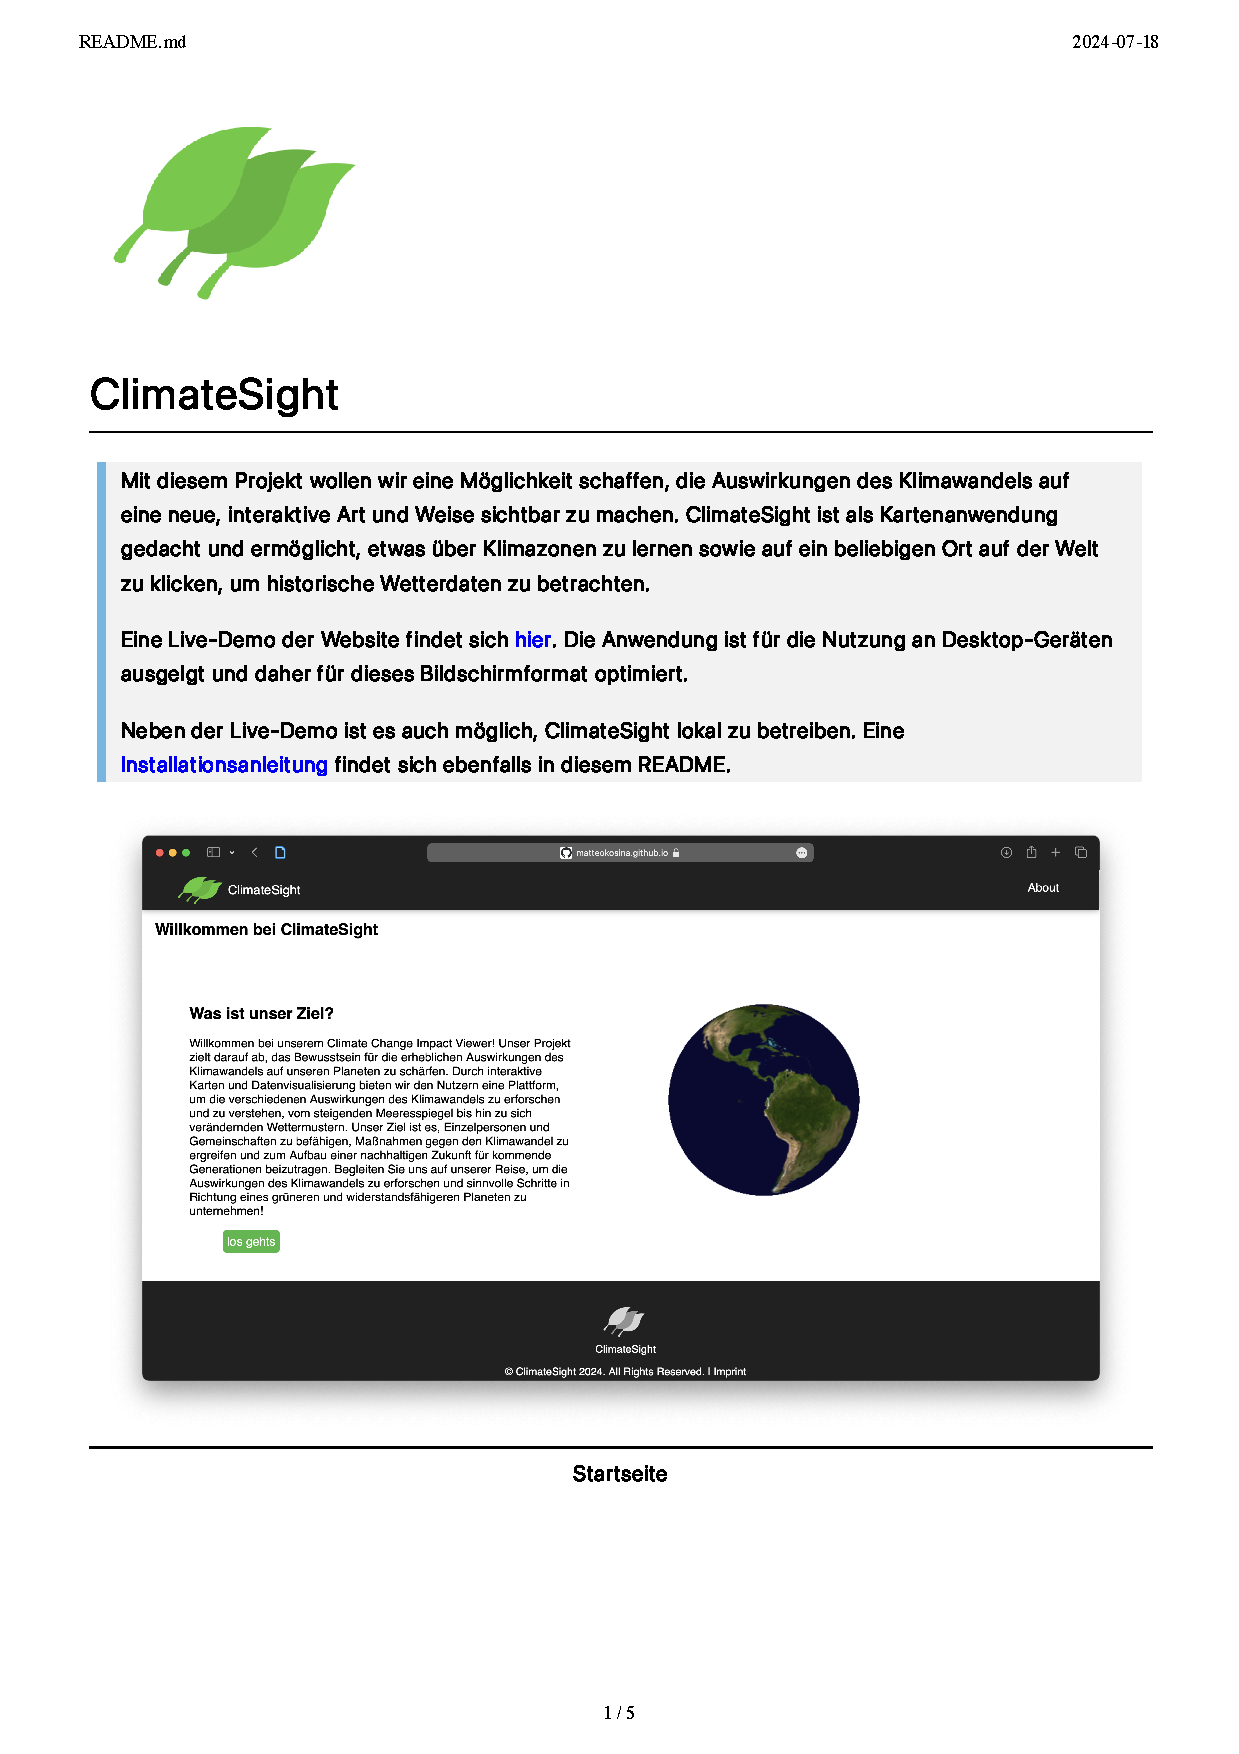
\includegraphics[width=\textwidth, page=1]{Planungsdokumente/graphics/README.pdf}
\includegraphics[width=\textwidth, page=2]{Planungsdokumente/graphics/README.pdf}
\includegraphics[width=\textwidth, page=3]{Planungsdokumente/graphics/README.pdf}
\includegraphics[width=\textwidth, page=4]{Planungsdokumente/graphics/README.pdf}
\includegraphics[width=\textwidth, page=5]{Planungsdokumente/graphics/README.pdf}
\includegraphics[width=\textwidth, page=6]{Planungsdokumente/graphics/README.pdf}

\section{Protokolle}
{\it Autor: Leon Fertig}
\newline
Für die Protokollierung ist eine Vorlage entworfen worden, nach der die Treffen jeweils protokolliert worden sind. Zwei Beispiele finden sich nachfolgend.
\newline
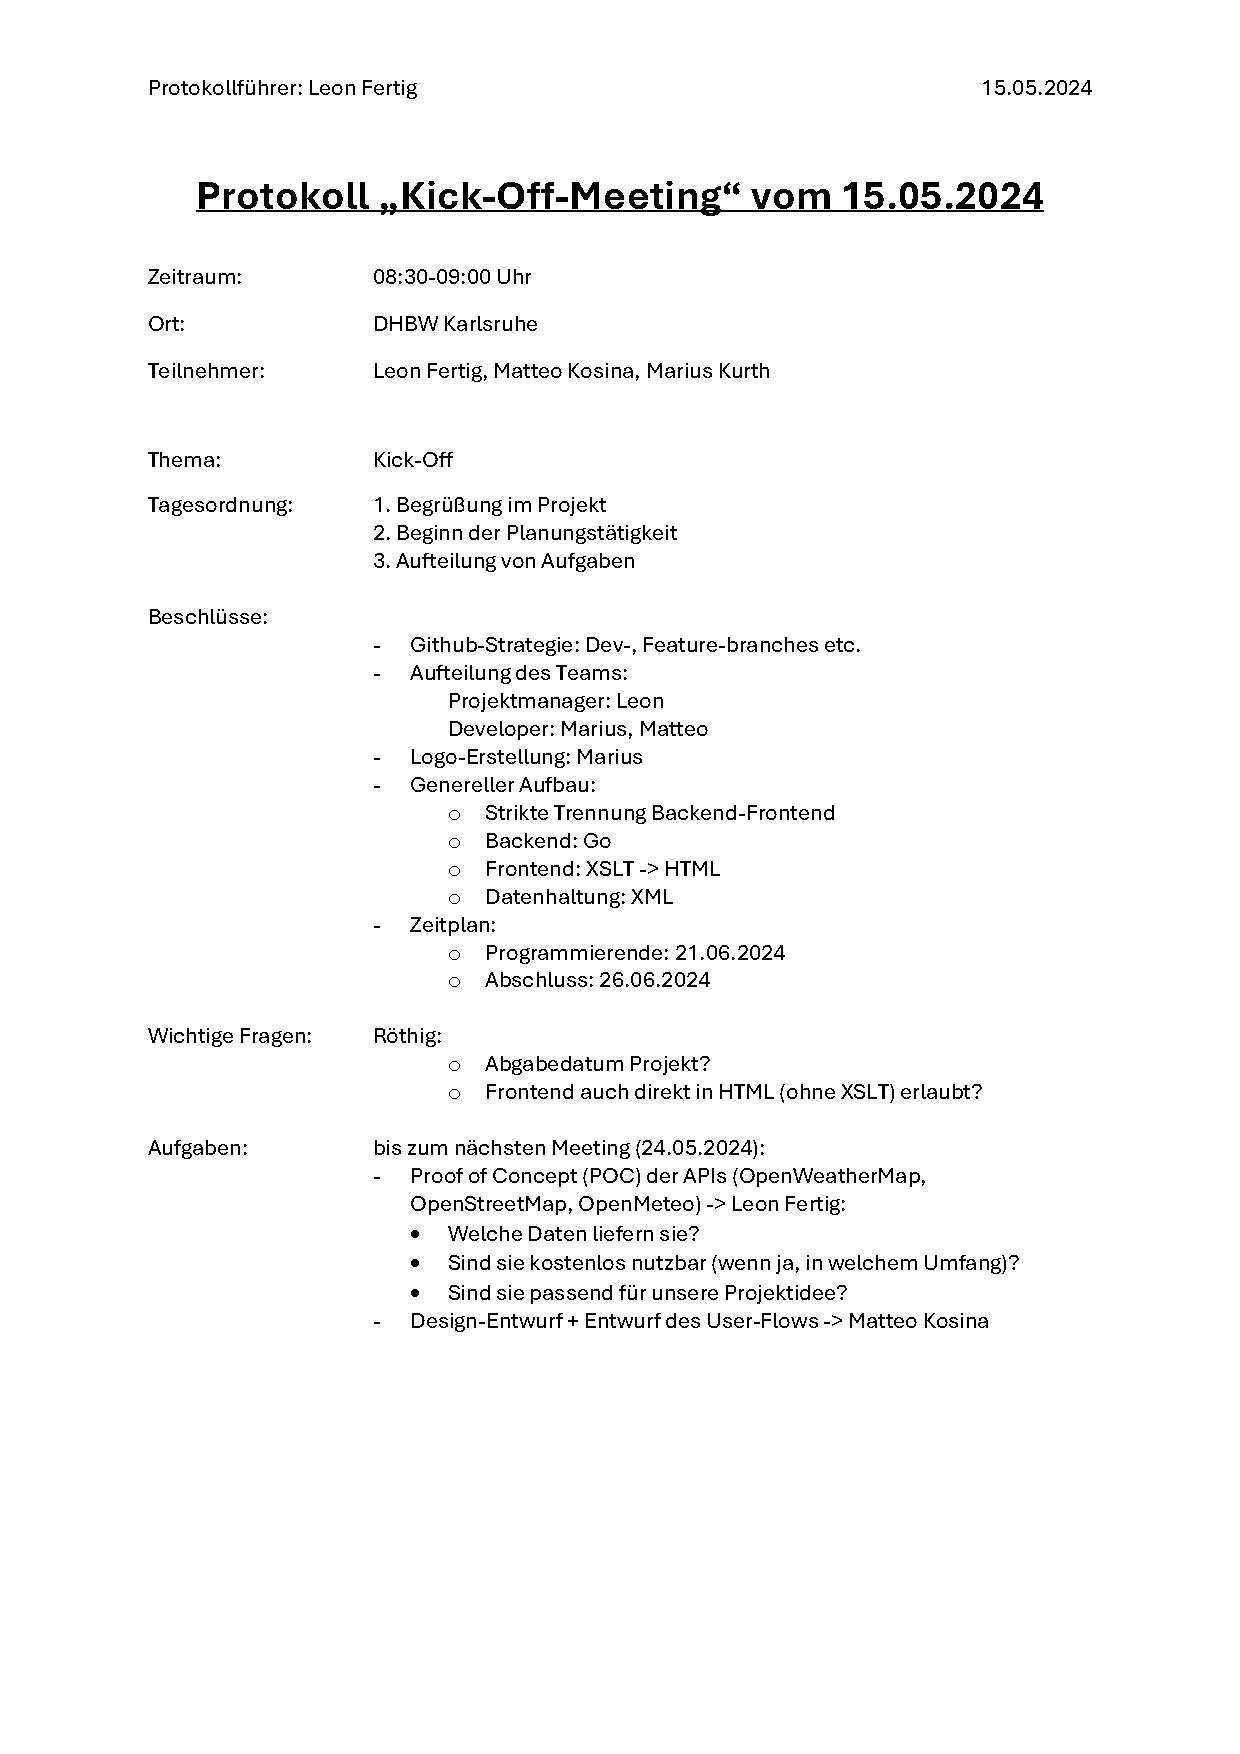
\includegraphics[width=\textwidth]{Planungsdokumente/graphics/Protokoll1.pdf}
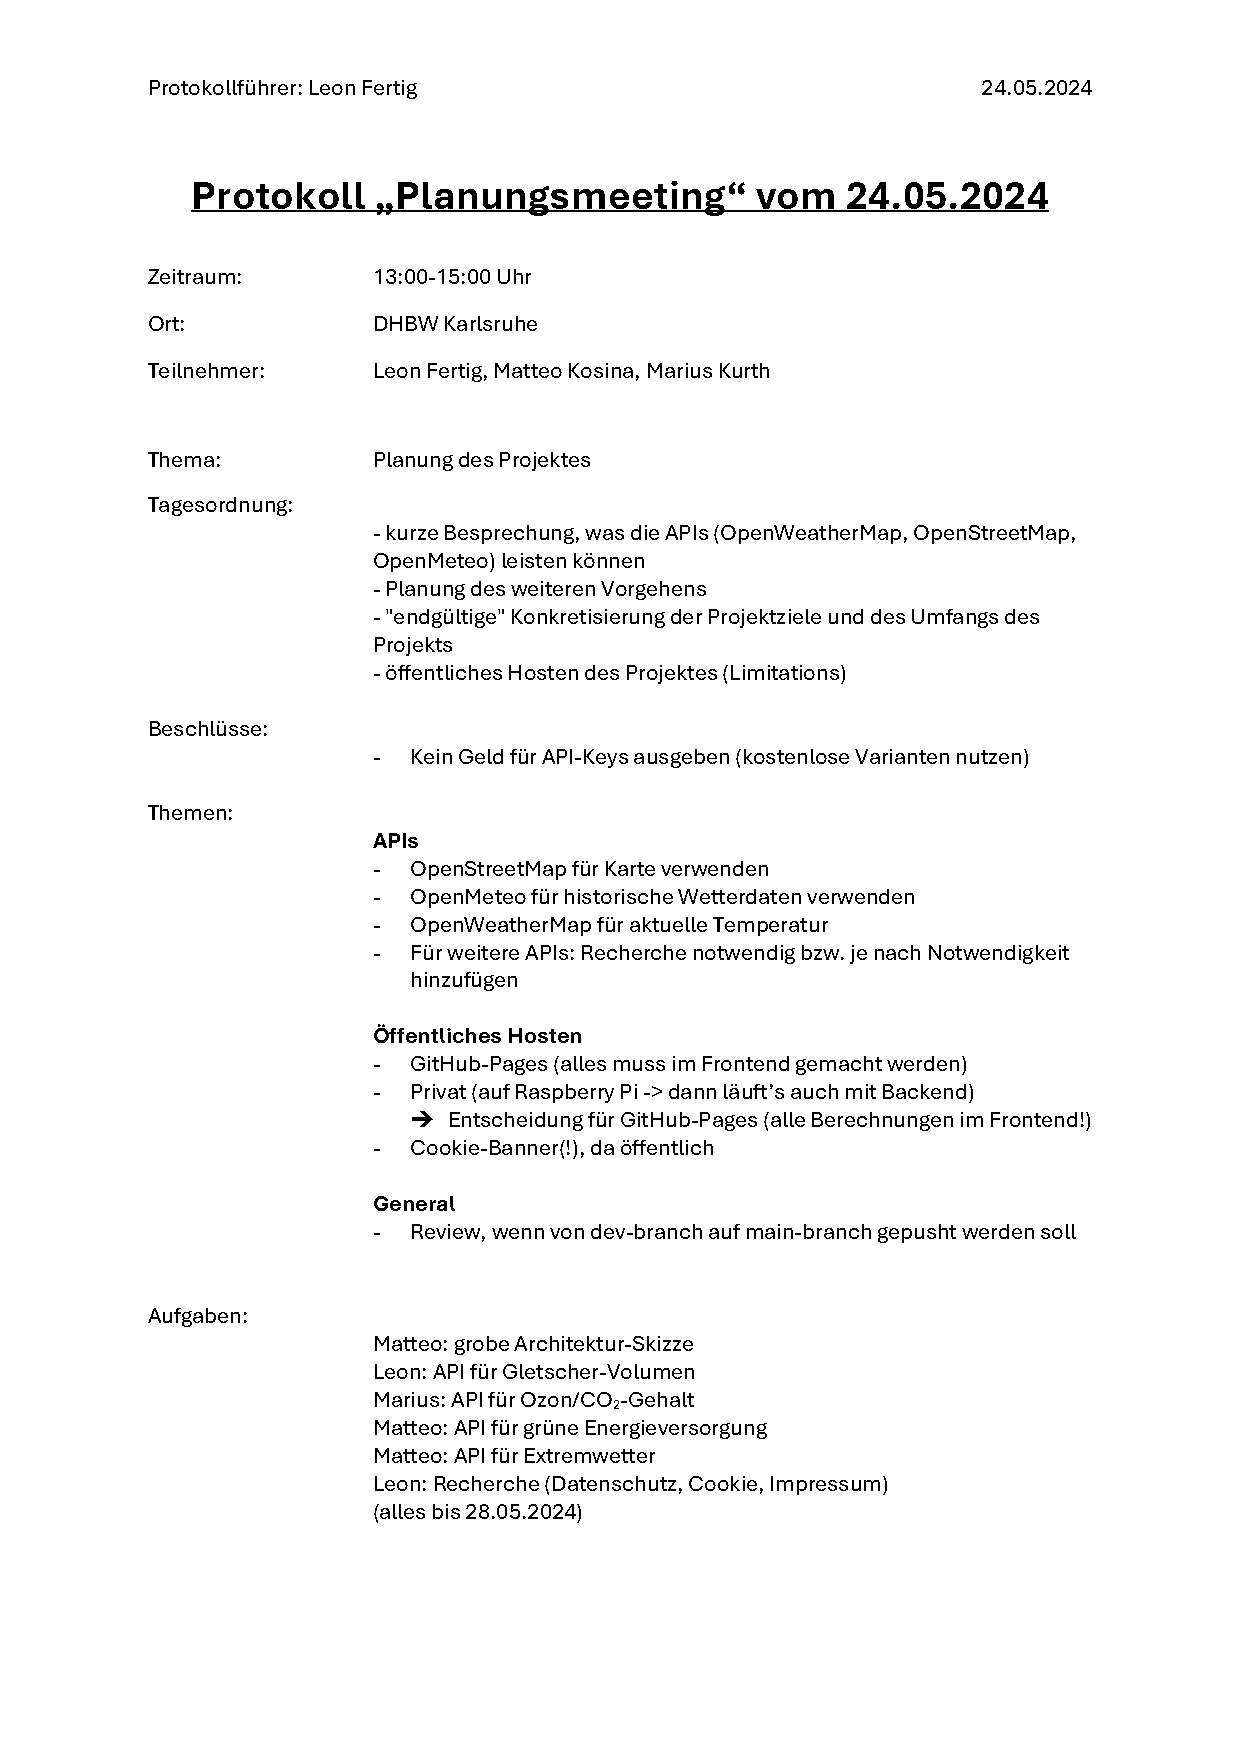
\includegraphics[width=\textwidth]{Planungsdokumente/graphics/Protokoll2.pdf}

\section{Projektauftrag}
{\it Autor: Leon Fertig}
\newline
Der Projektauftrag geht aus den Anforderungen des Auftraggebers Herrn Röthig hervor und gibt wieder, was der Auftraggeber von uns erwartet. Das Projektgesamtziel, die Teilziele und die Rahmenbedingungen und der Projektkontext sind direkt aus den Anforderungen von Herrn Röthig zitiert.
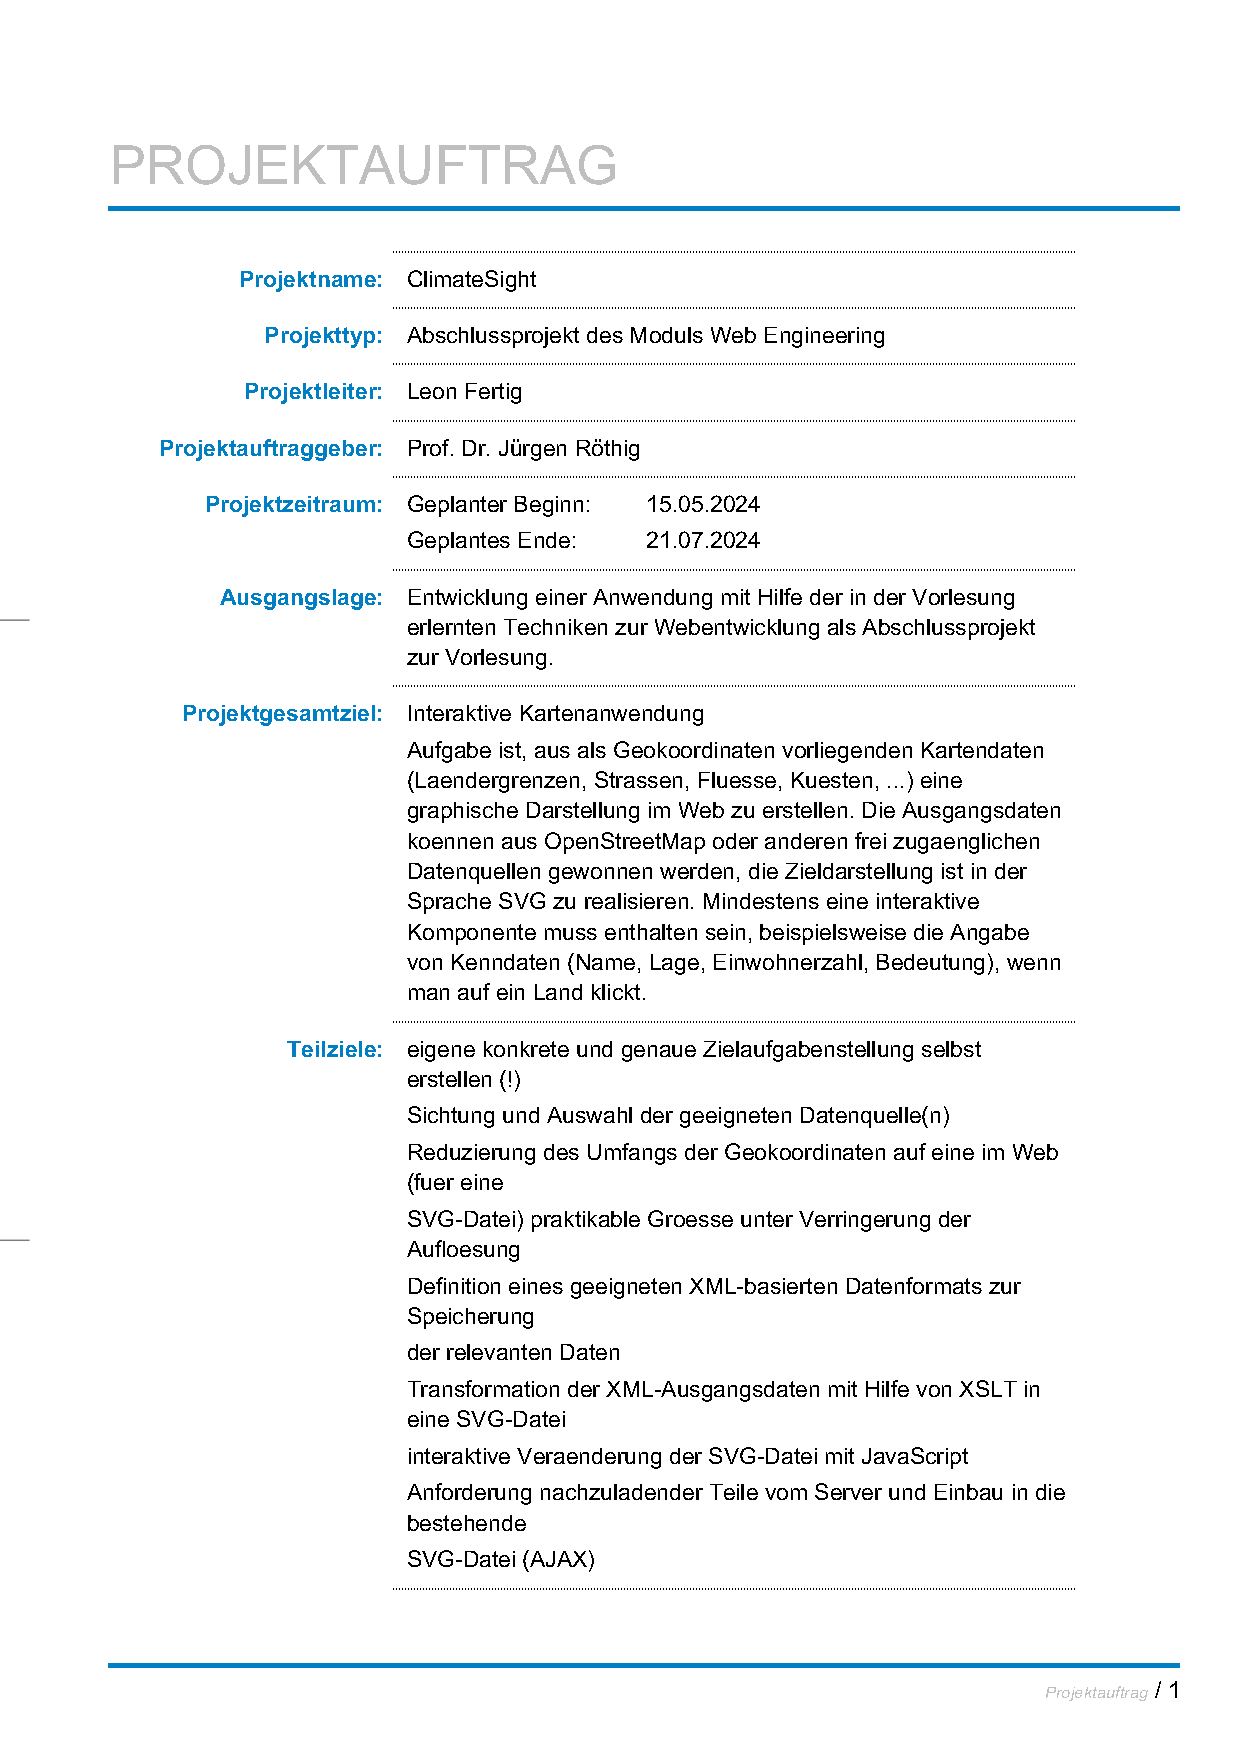
\includepdf[pages=-]{Planungsdokumente/graphics/Projektauftrag.pdf}

\section{Projektziele}
{\it Autor: Matteo Kosina}
\newline
\subsection*{Muss-Kriterien}
\begin{itemize}
	\item Es werden verschiedene Datenquelle (APIs) für Klimadaten angeschaut und analysiert, welche nützlich für das Projekt sein können. Dabei muss beachtet werden, dass kein Budget für API-Keys zur Verfügung steht, die in Frage kommenden Datenquellen müssen also kostenlos sein.
    \item Es wird eine Web-Applikation für Desktop-PCs entwickelt mit folgenden Komponenten:
    \begin{itemize}
		\item Eine Landing-Page, auf der ein kurzer Text mit Beschreibungen zu dem Projekt zu finden sind und ein Button, der den User auf die Discover-Page weiterleitet
		\item Eine Discover-Page, auf der eine Karte zu sehen ist. Beim Klick auf ein Land wird der User auf die Analytics-Page des entsprechenden Landes weitergeleitet.
		\item Eine Analytics-Page für jedes Land der Erde, die die Hauptstadt, die Flagge und die aktuelle Einwohnerzahl des Landes anzeigt. Außerdem zeigt diese Seite die aktuelle Temperatur und historische Wetterdaten für Temperatur und Niederschlag an.
	\end{itemize}
    \item Es wird eine Installationsanleitung erstellt, die es einem Administrator erlaubt, den Webserver bei sich zu betreiben. Eine Demo-Installation mit einem einfachen Python-Webserver wird Schritt für Schritt beschrieben. Für die produktive Nutzung werden jedoch einige Kenntnisse benötigt, die die Installationsanleitung nicht bereitstellt.
    \item Für die Datenspeicherung wird XML verwendet (API-Daten müssen gegebenenfalls von JSON in XML umgewandelt werden). Mithilfe von XSLT werden diese Daten in HTML oder SVG umgewandelt. Hierfür werden geeignete Datenformate definiert.
\end{itemize}

\subsection*{Soll-Kriterien}
\begin{itemize}
    \item Die Sprache kann zwischen Deutsch und Englisch gewechselt werden.
    \item Auf der Analytics-Page werden lokale Nachrichten (mit Fokus auf Klima + Wetter) angezeigt.
    \item Auf der Discover-Page kann man mit einem Klimafilter (nach Temperatur und/oder Niederschlag) die Länder gruppieren, um eine bessere Übersichtlichkeit zu erreichen.
\end{itemize}

\subsection*{Kann-Kriterien}
\begin{itemize}
    \item Der User kann zwischen verschiedenen Kartenansichten auswählen: Satellit, geographisch, Heat-Map
\end{itemize}

\subsection*{Abgrenzungskriterien}
\begin{itemize}
    \item kein Einsatz von KI
    \item keine Routenführung
    \item keine mobile Anwendung (nicht für Smartphone oder Tablets optimiert)
\end{itemize}

\section{Phasen- und Meilensteinplan}
{\it Autor: Leon Fertig}
\newline
Der Phasen- und Meilensteinplan enthält {\bf nicht} die Arbeitspakete aus Projektstrukturplan, Gantt-Diagramm etc., da die Arbeitspakete - der geringen Größe des Projekts geschuldet - relativ viele kleineren Aufgaben enthalten und daher über relativ große Zeiträume reichen, sodass ein übersichtlicher Phasen- und Meilensteinplan nicht möglich wäre. Daher wurde der Phasen- und Meilensteinplan als grobe Übersicht erstellt und das Gantt-Diagramm wurde zur Überprüfung des Zeitplans eingesetzt.
\newline
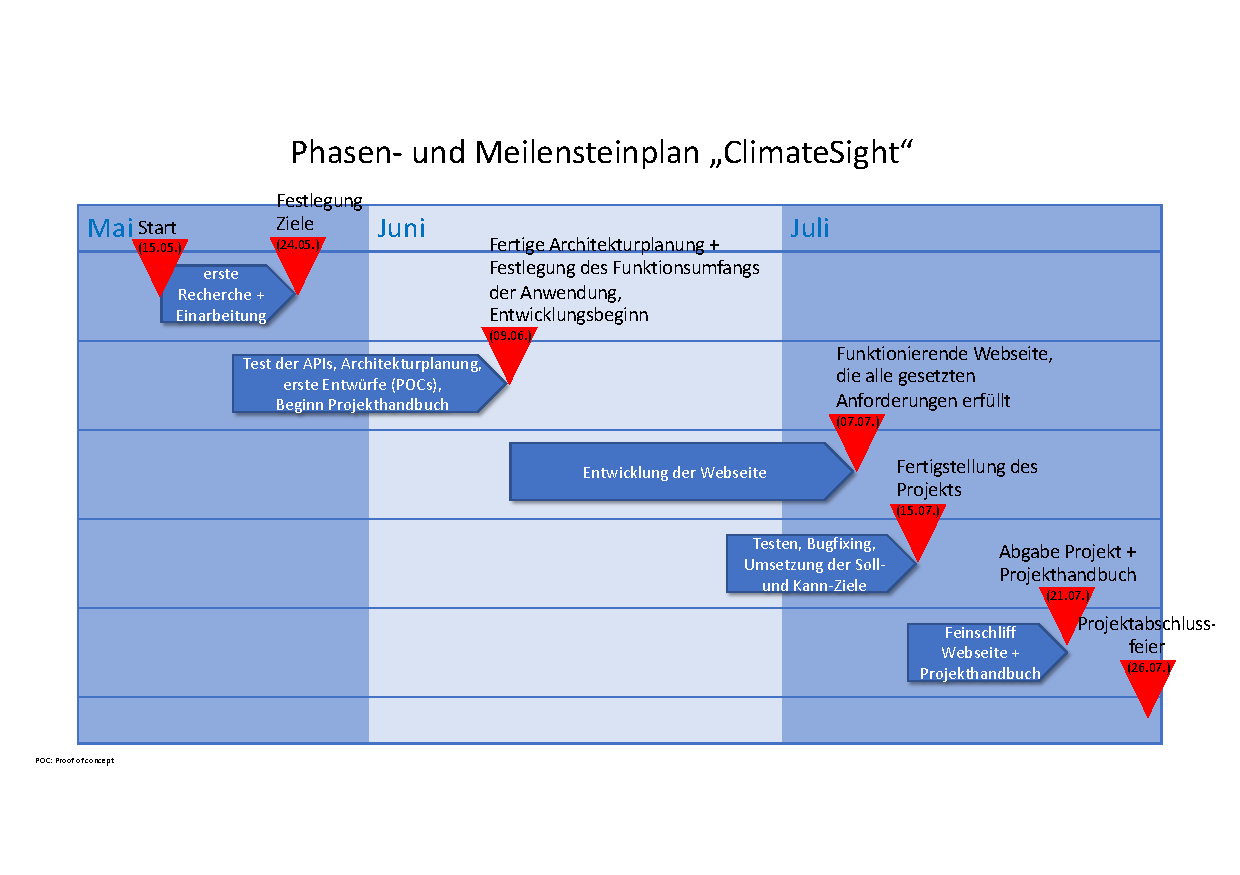
\includegraphics[width=\textwidth]{Planungsdokumente/graphics/Meilensteinplan.pdf}

\section{Projektorganigramm}
{\it Autor: Matteo Kosina}
\newline
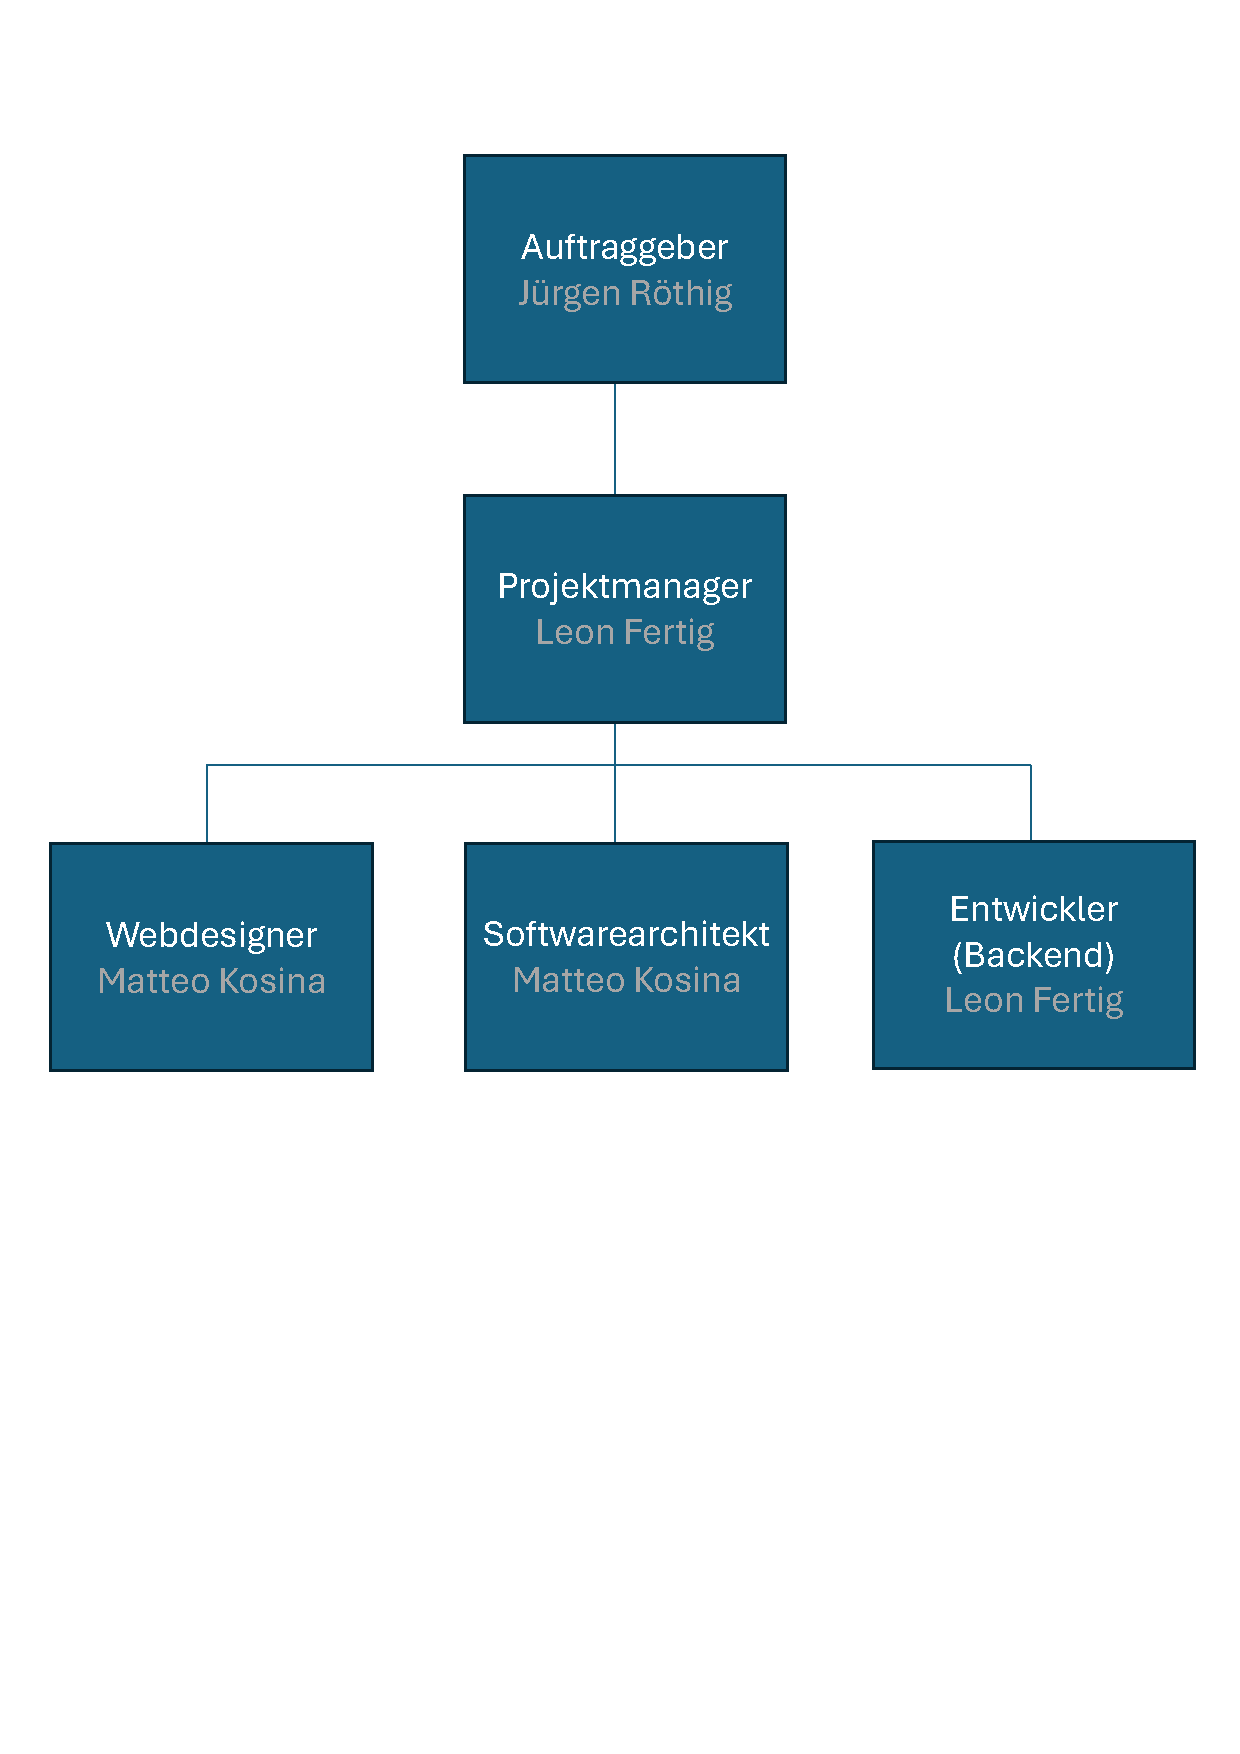
\includegraphics[width=\textwidth]{Planungsdokumente/graphics/Projektorganigramm.pdf}

\section{Offene-Punkte-Liste OPL}
{\it Autor: Leon Fertig}
\newline
Offene Punkteliste zum 04.06.2024.
Die Aufgaben aus der OPL stimmen nicht immer zu 100\% mit denen der Protokolle überein, da sie teilweise nachträglich noch geändert (oder die Termine nach hinten verschoben) werden mussten, sodass die Protokolle keine aktuelle Version der Aufgaben darstellen, sondern {\bf nur} die OPL!
\newline
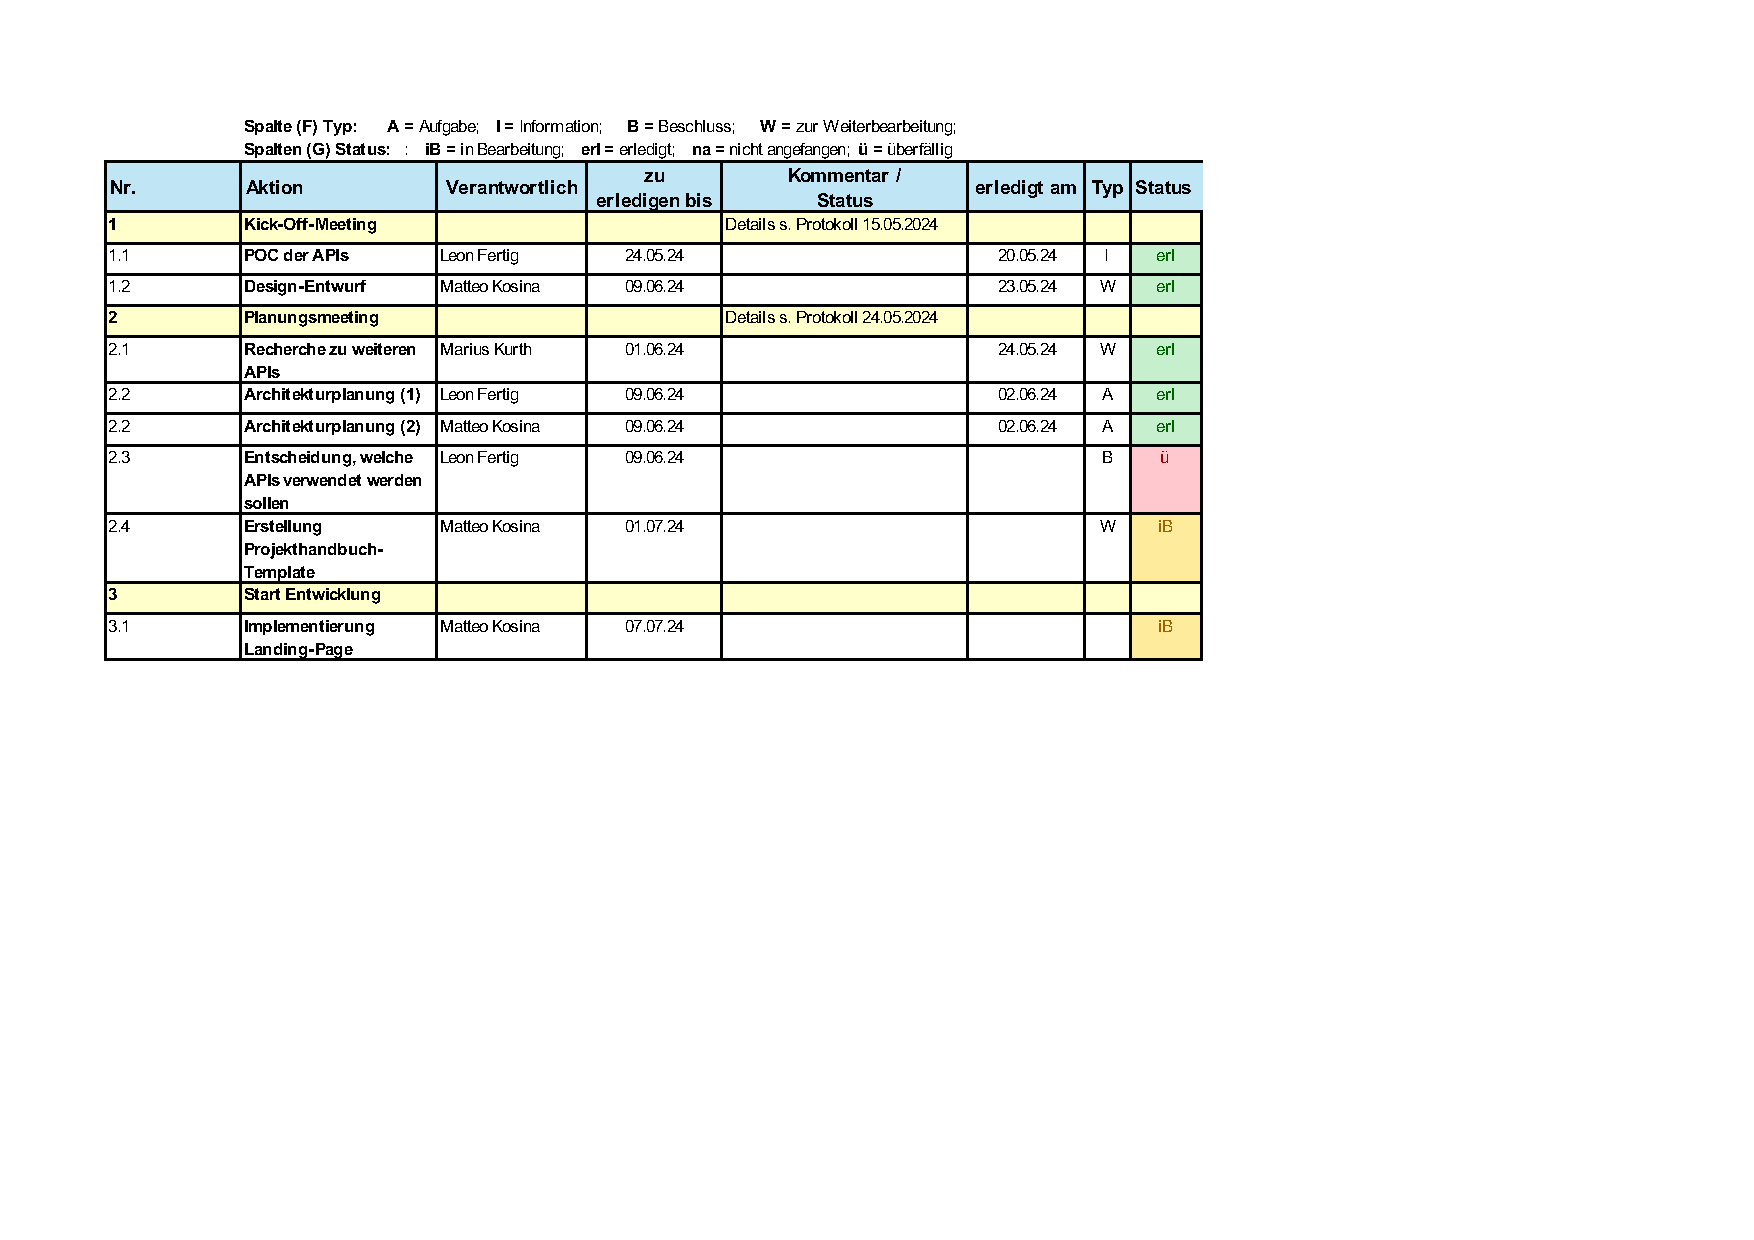
\includegraphics[width=\textwidth]{Planungsdokumente/graphics/Offene_Punkteliste.pdf}

\section{Projektstrukturplan}
{\it Autor: Matteo Kosina}
\newline
Es wurde eine Gemischter Projektstrukturplan erstellt:
\begin{itemize}
	\item {\bf Projektmanagement}: Mischung aus Objektorientierung und Phasenorientierung
	\item {\bf Frontend}: Objektorientierung (wobei die Überarbeitung von UX + Design eher einem phasenorientierten Ansatz entspricht)
	\item {\bf Backend}: phasenorientiert
\end{itemize}
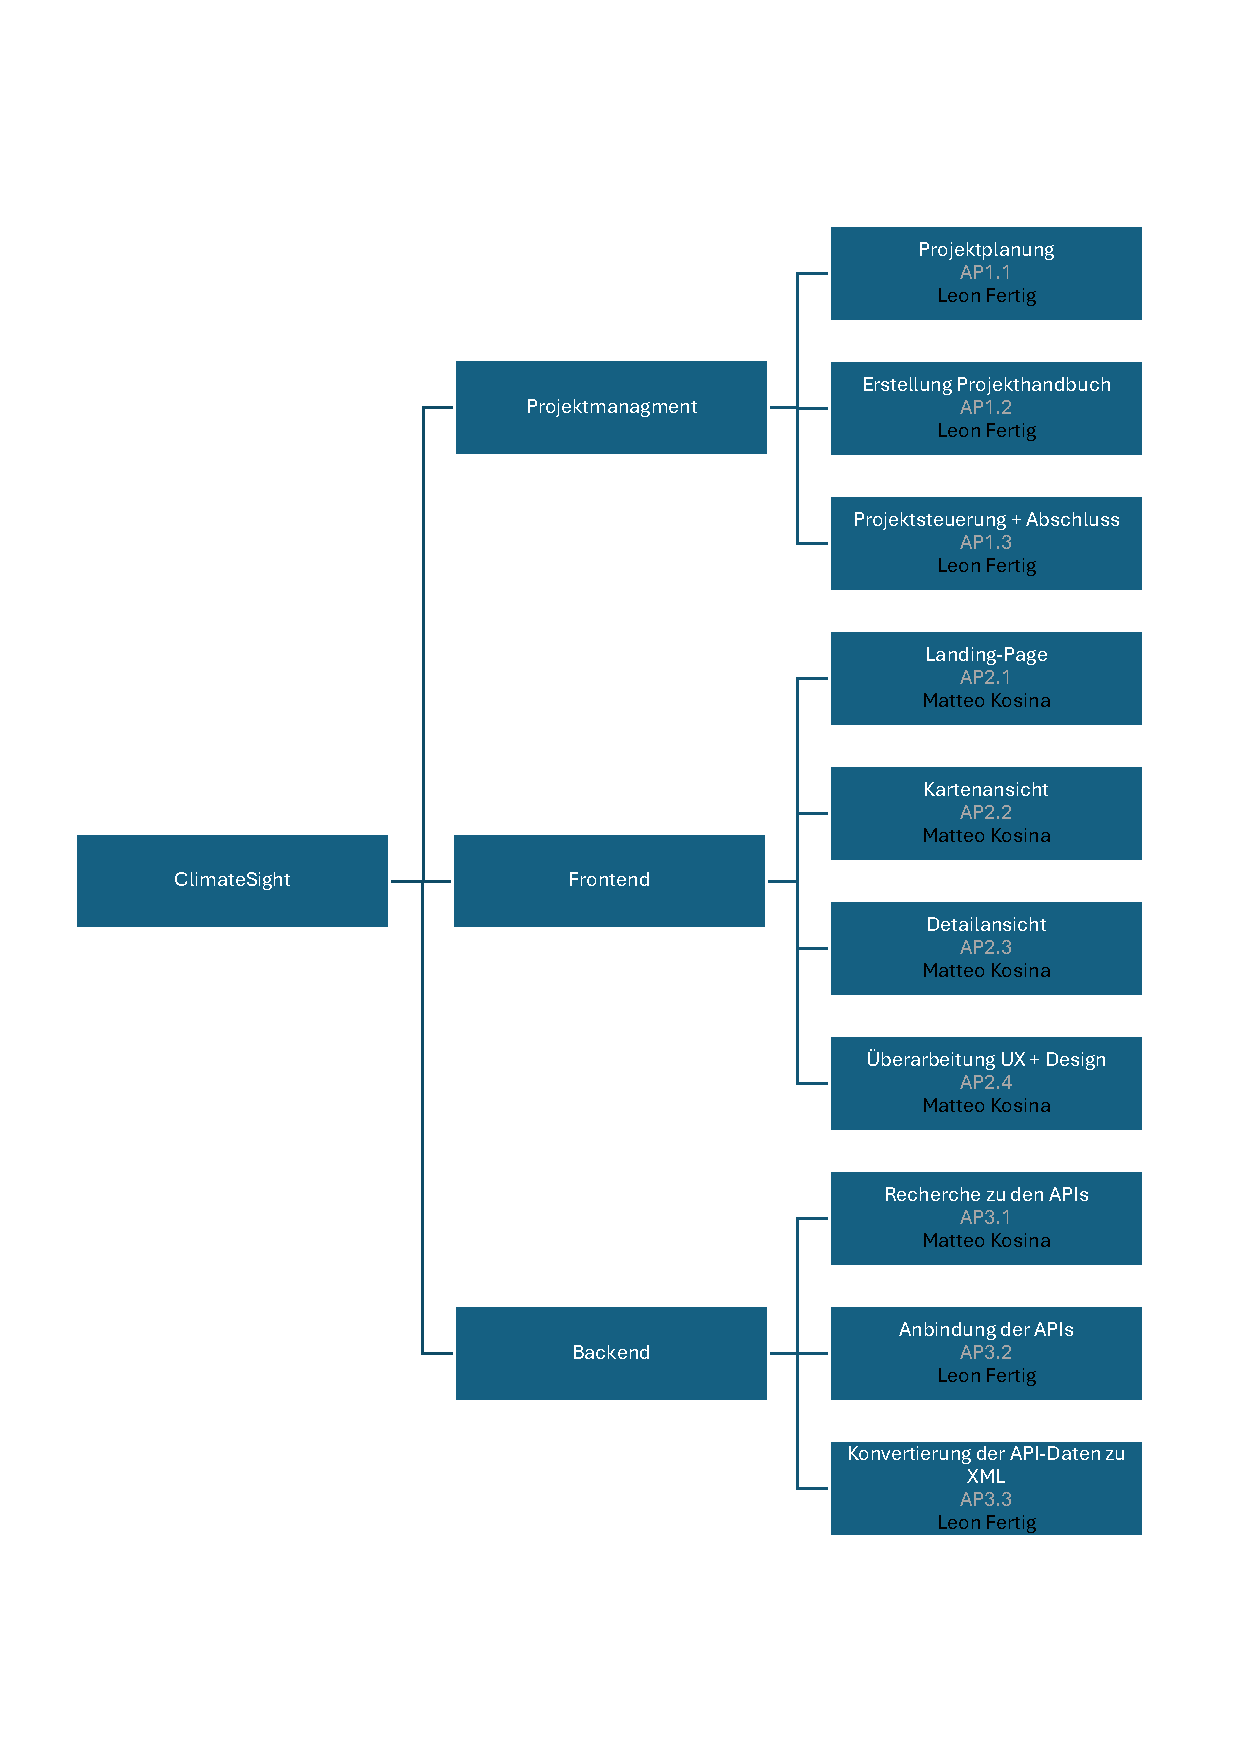
\includegraphics[width=\textwidth]{Planungsdokumente/graphics/Projektstrukturplan.pdf}

\section{Arbeitspaketbeschreibungen}
{\it Autor: jeweils AP-Verantwortlicher}
\newline
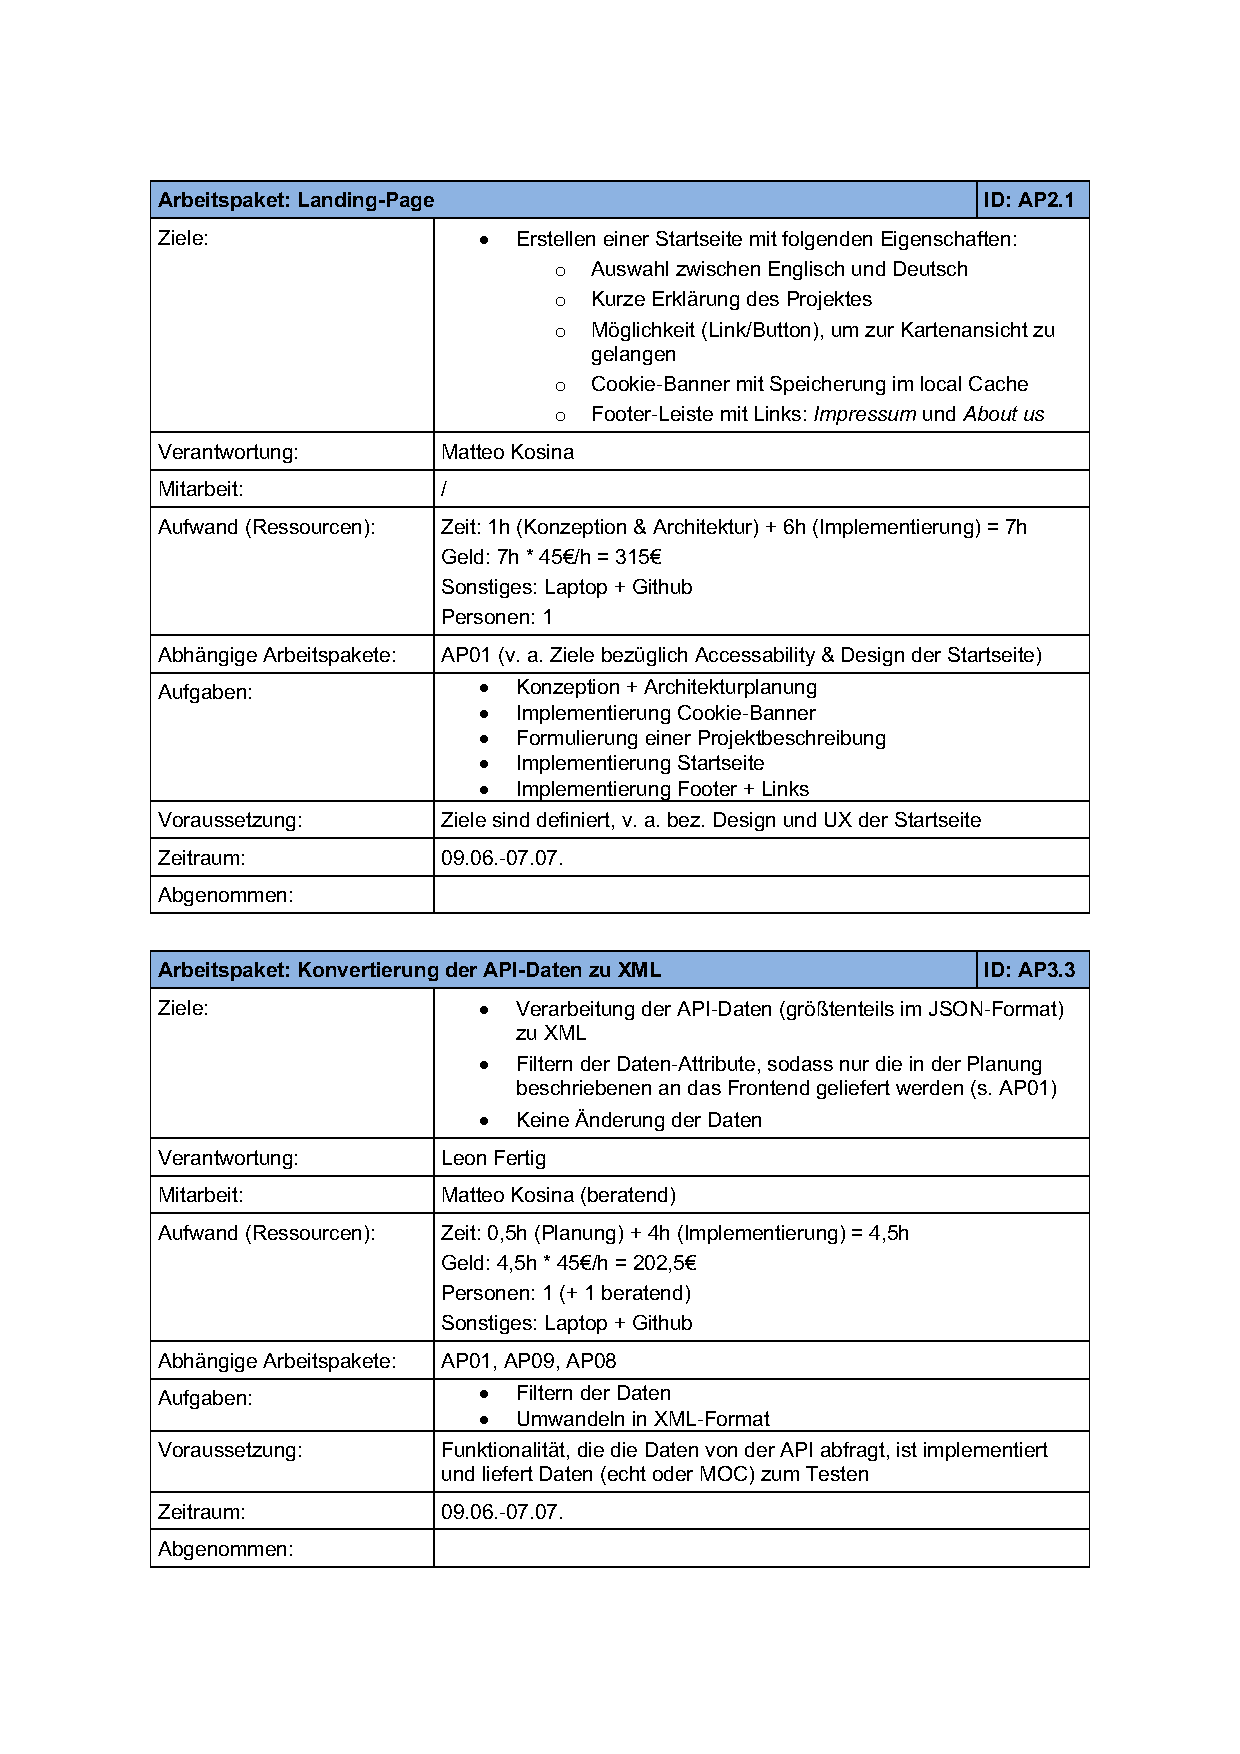
\includegraphics[width=\textwidth]{Planungsdokumente/graphics/Arbeitspakete.pdf}

\section{Gantt-Diagramm}
{\it Autor: Leon Fertig}
\newline
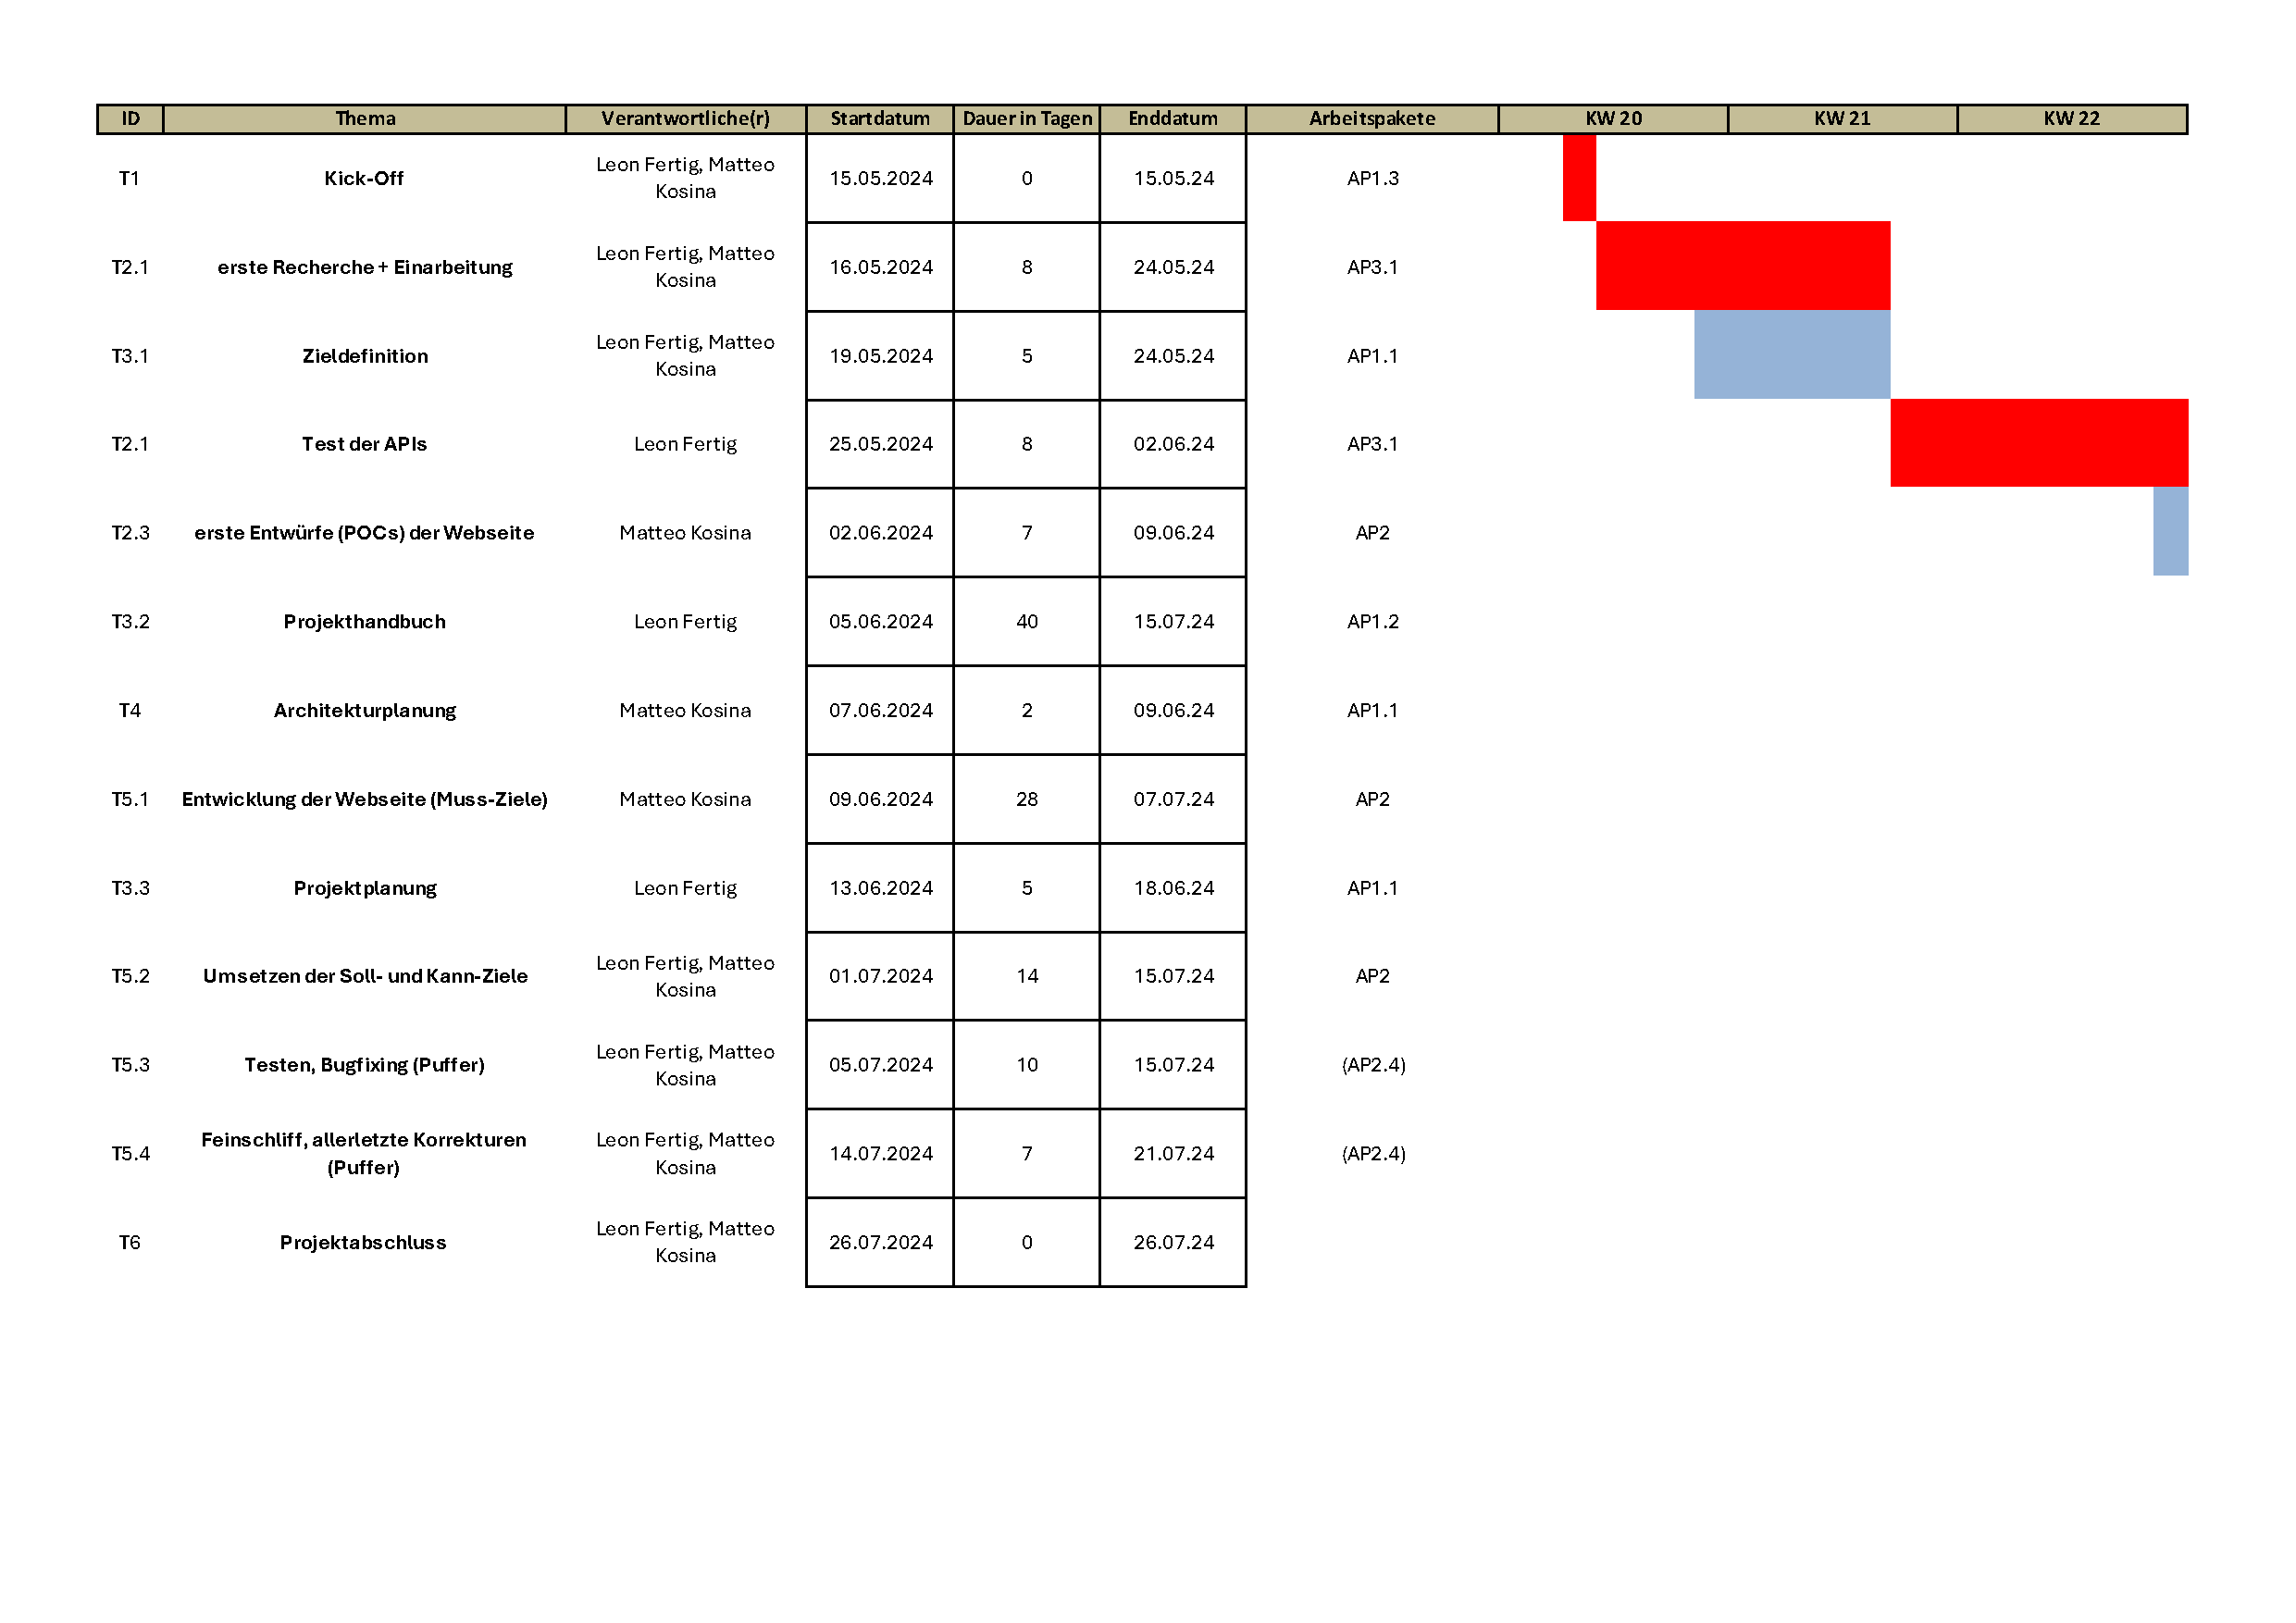
\includegraphics[width=\textwidth, page=1]{Planungsdokumente/graphics/Gantt_Diagramm.pdf}
\pagebreak

\section{Ressourcen- und Kostenplan}
{\it Autor: Matteo Kosina}
\newline
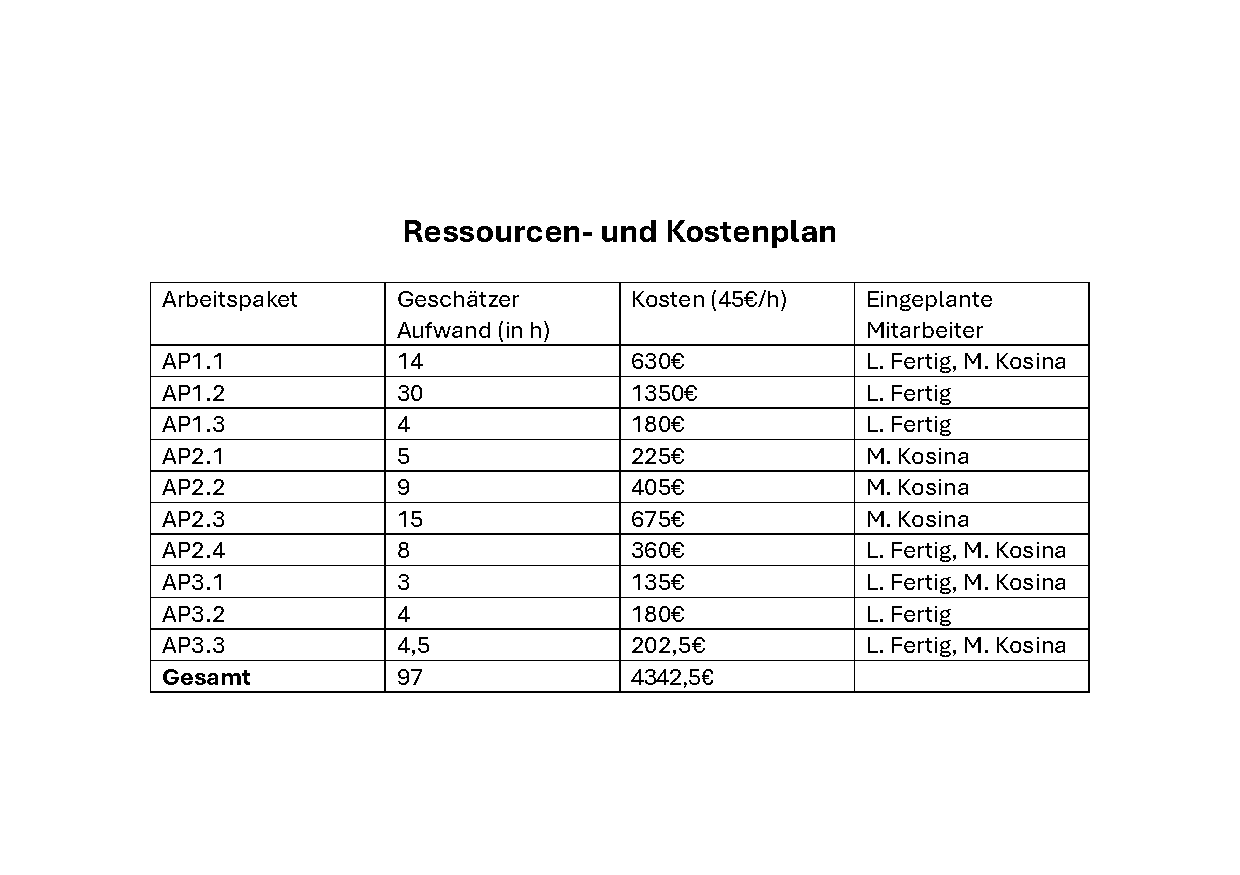
\includegraphics[width=\textwidth]{Planungsdokumente/graphics/Ressourcenplan.pdf}

\section{Risikoanalyse}
{\it Autor: Matteo Kosina}
\newline
Es wurde die qualitative Risikobehandlung gewählt, da sie einen besseren Überblick über die Gefahren/Auswirkungen der einzelnen Risiken geben. Außerdem fehlt dem Team die Erfahrung für akkurate Geldwert-Einschätzungen, weshalb der Fokus nicht so stark auf Geldbeträge gelegt werden soll.
\newline
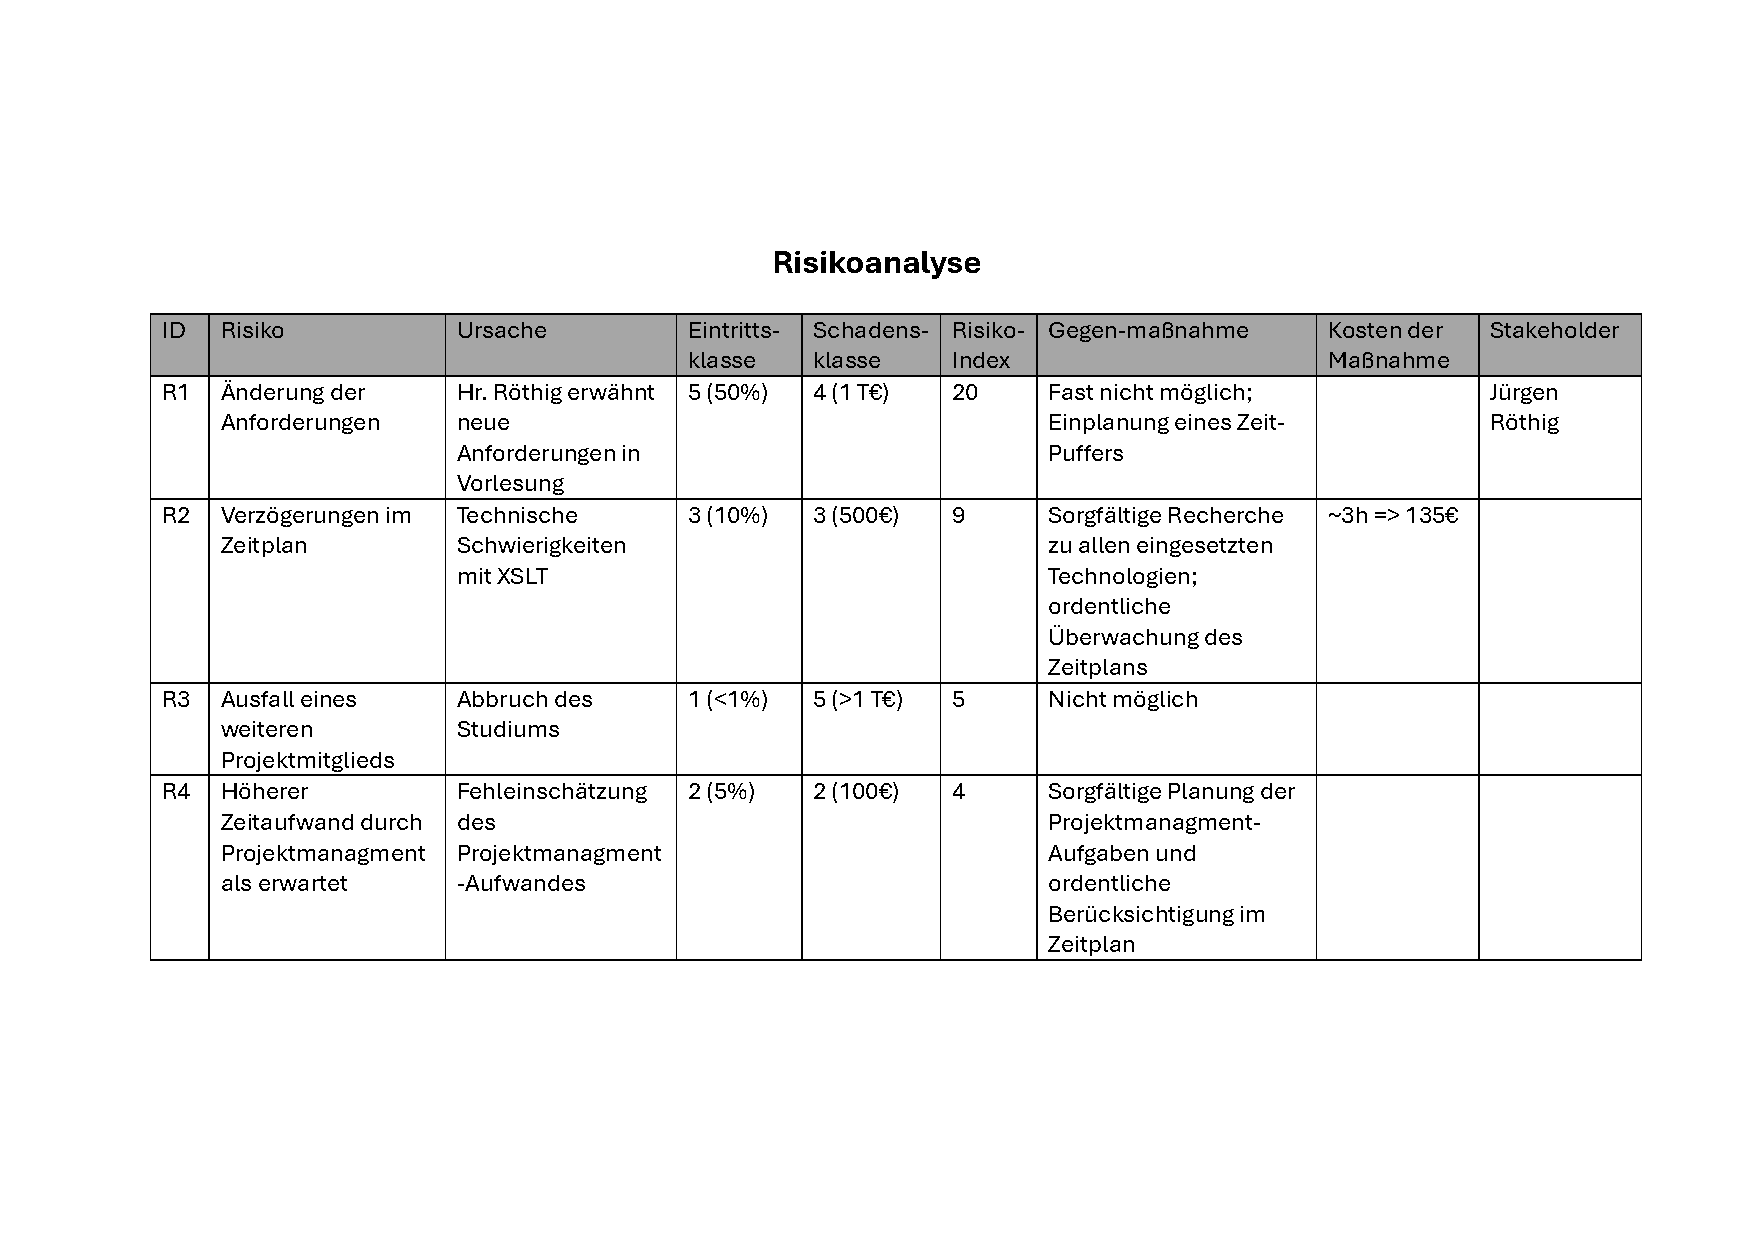
\includegraphics[width=\textwidth]{Planungsdokumente/graphics/Risikoanalyse.pdf}
\subsection*{Risikomatrix}
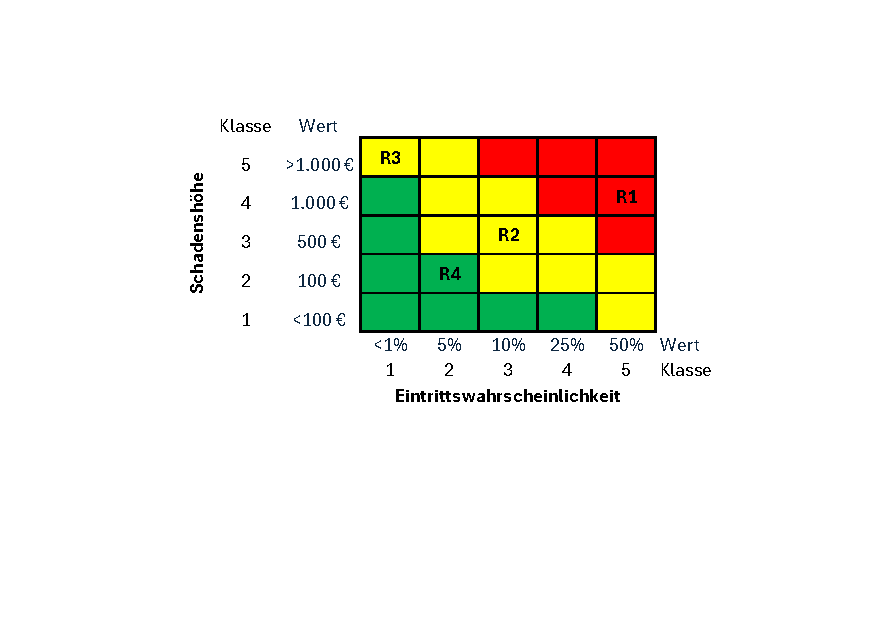
\includegraphics[width=\textwidth]{Planungsdokumente/graphics/Risikomatrix.pdf}

\section{Stakeholderanalyse}
{\it Autor: Matteo Kosina}
\newline
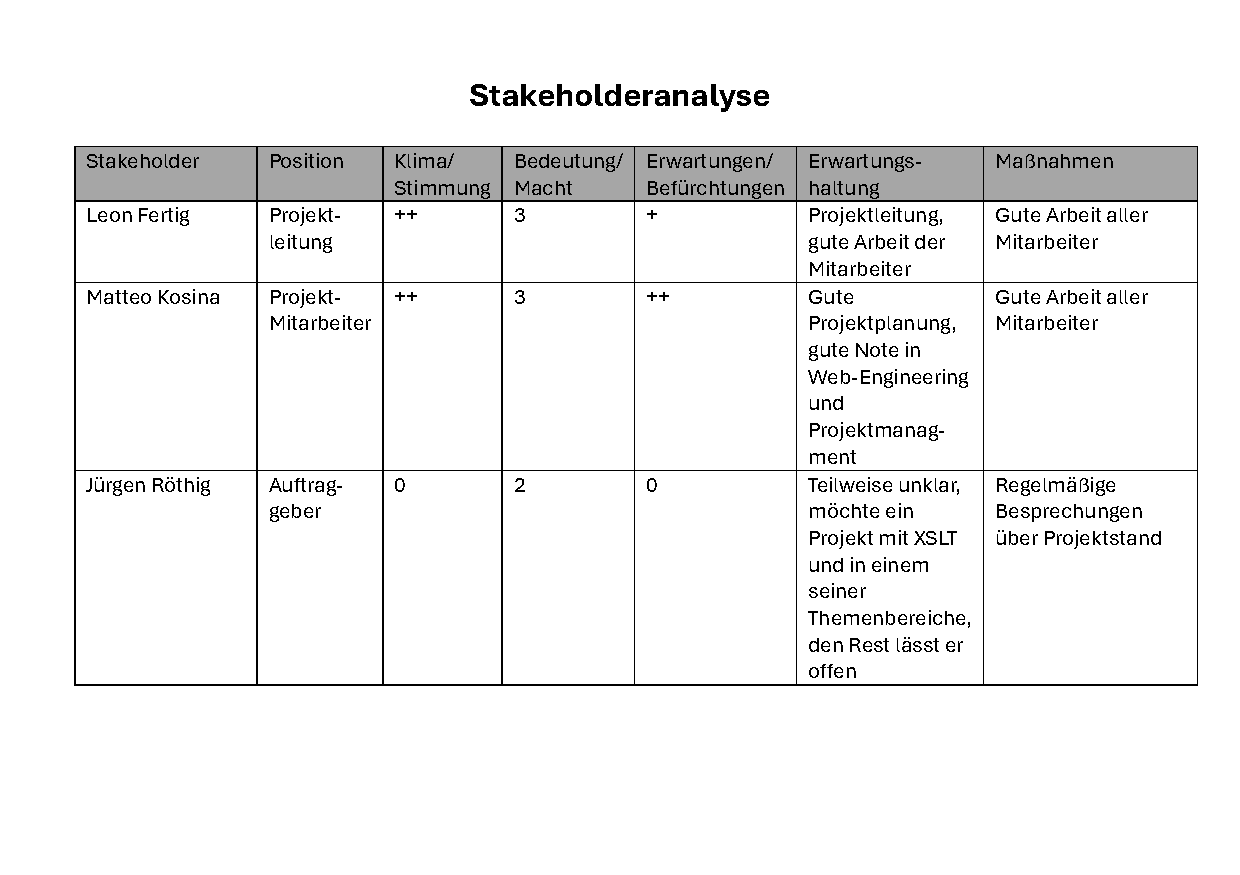
\includegraphics[width=\textwidth]{Planungsdokumente/graphics/Stakeholderanalyse.pdf}

\section{Projektstatusbericht}
{\it Autor: Leon Fertig}
\newline
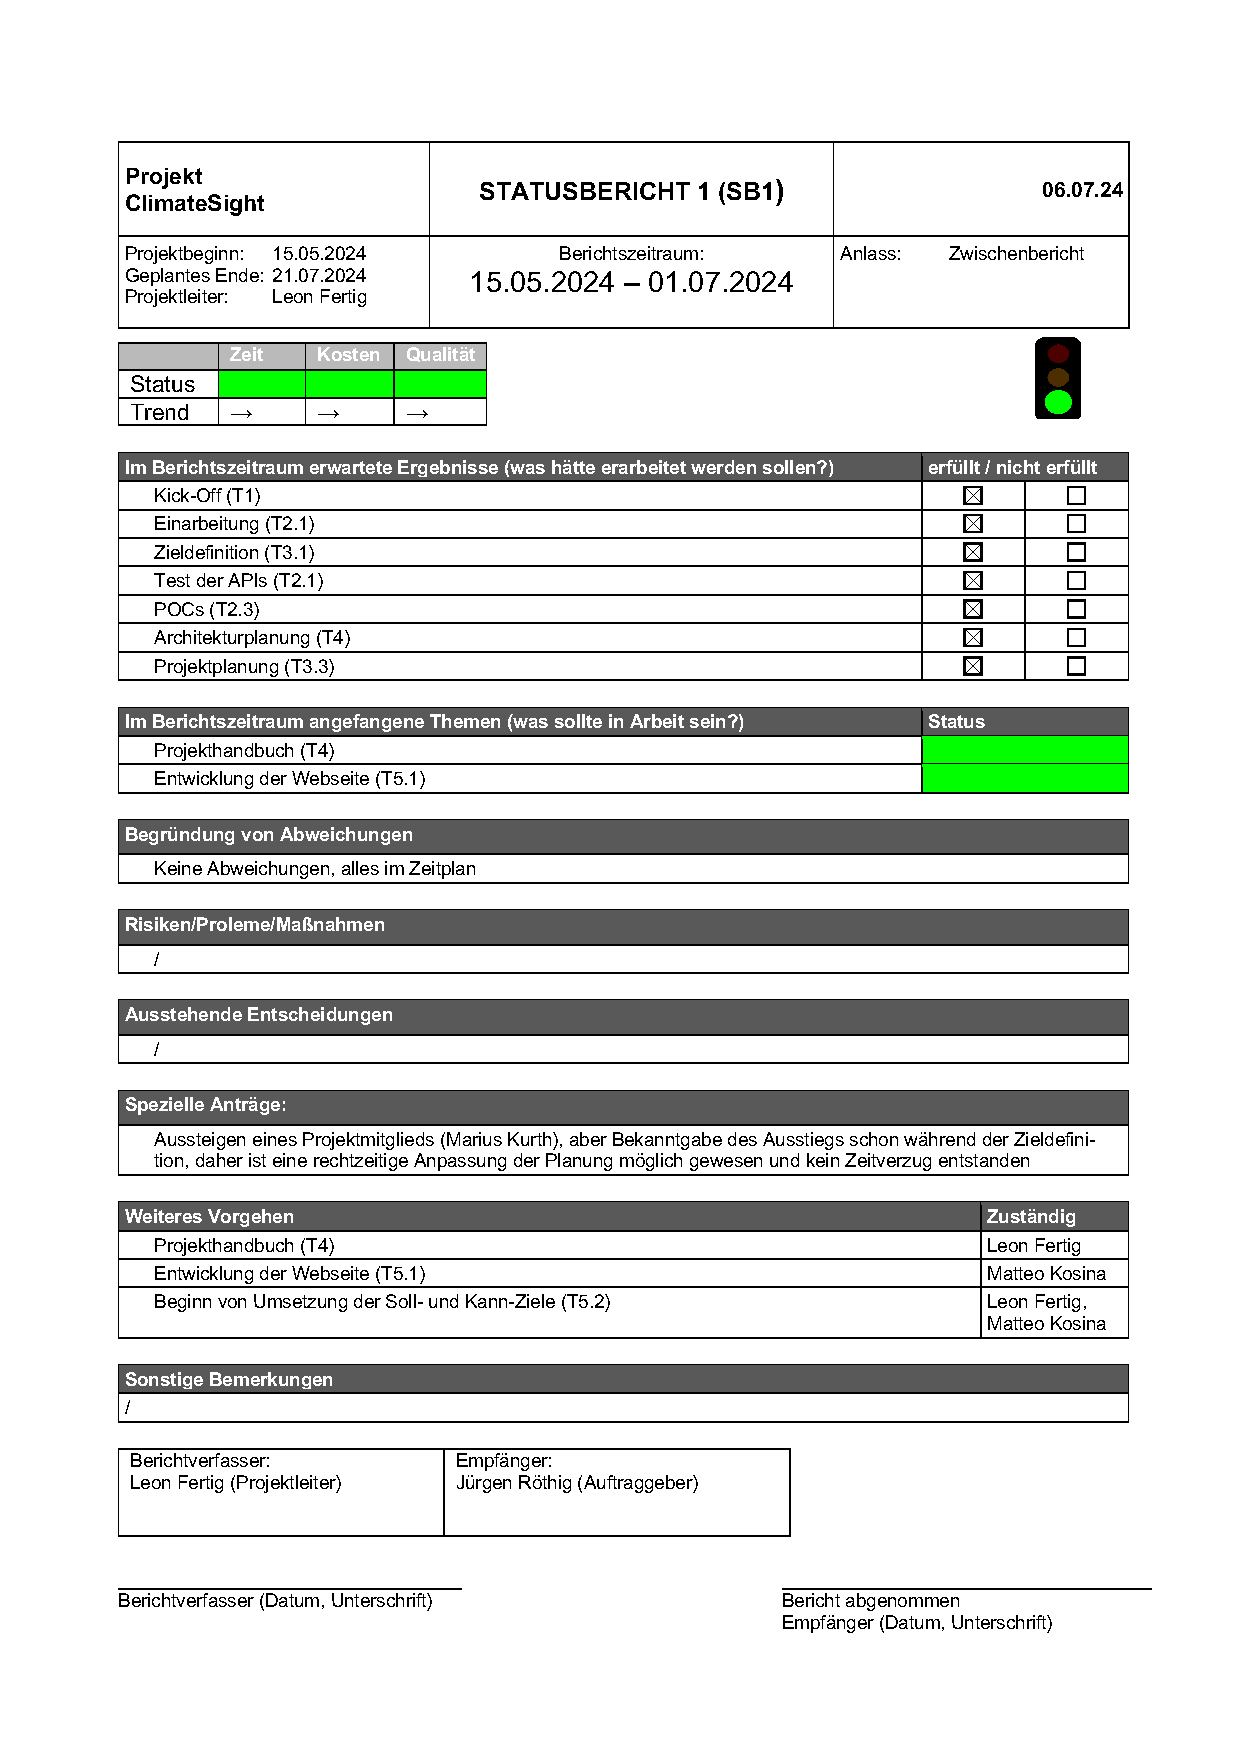
\includegraphics[width=\textwidth]{Planungsdokumente/graphics/Projektstatusbericht.pdf}

\section{Product Backlog und Sprint Backlog}
{\it Autor: Leon Fertig}
\newline
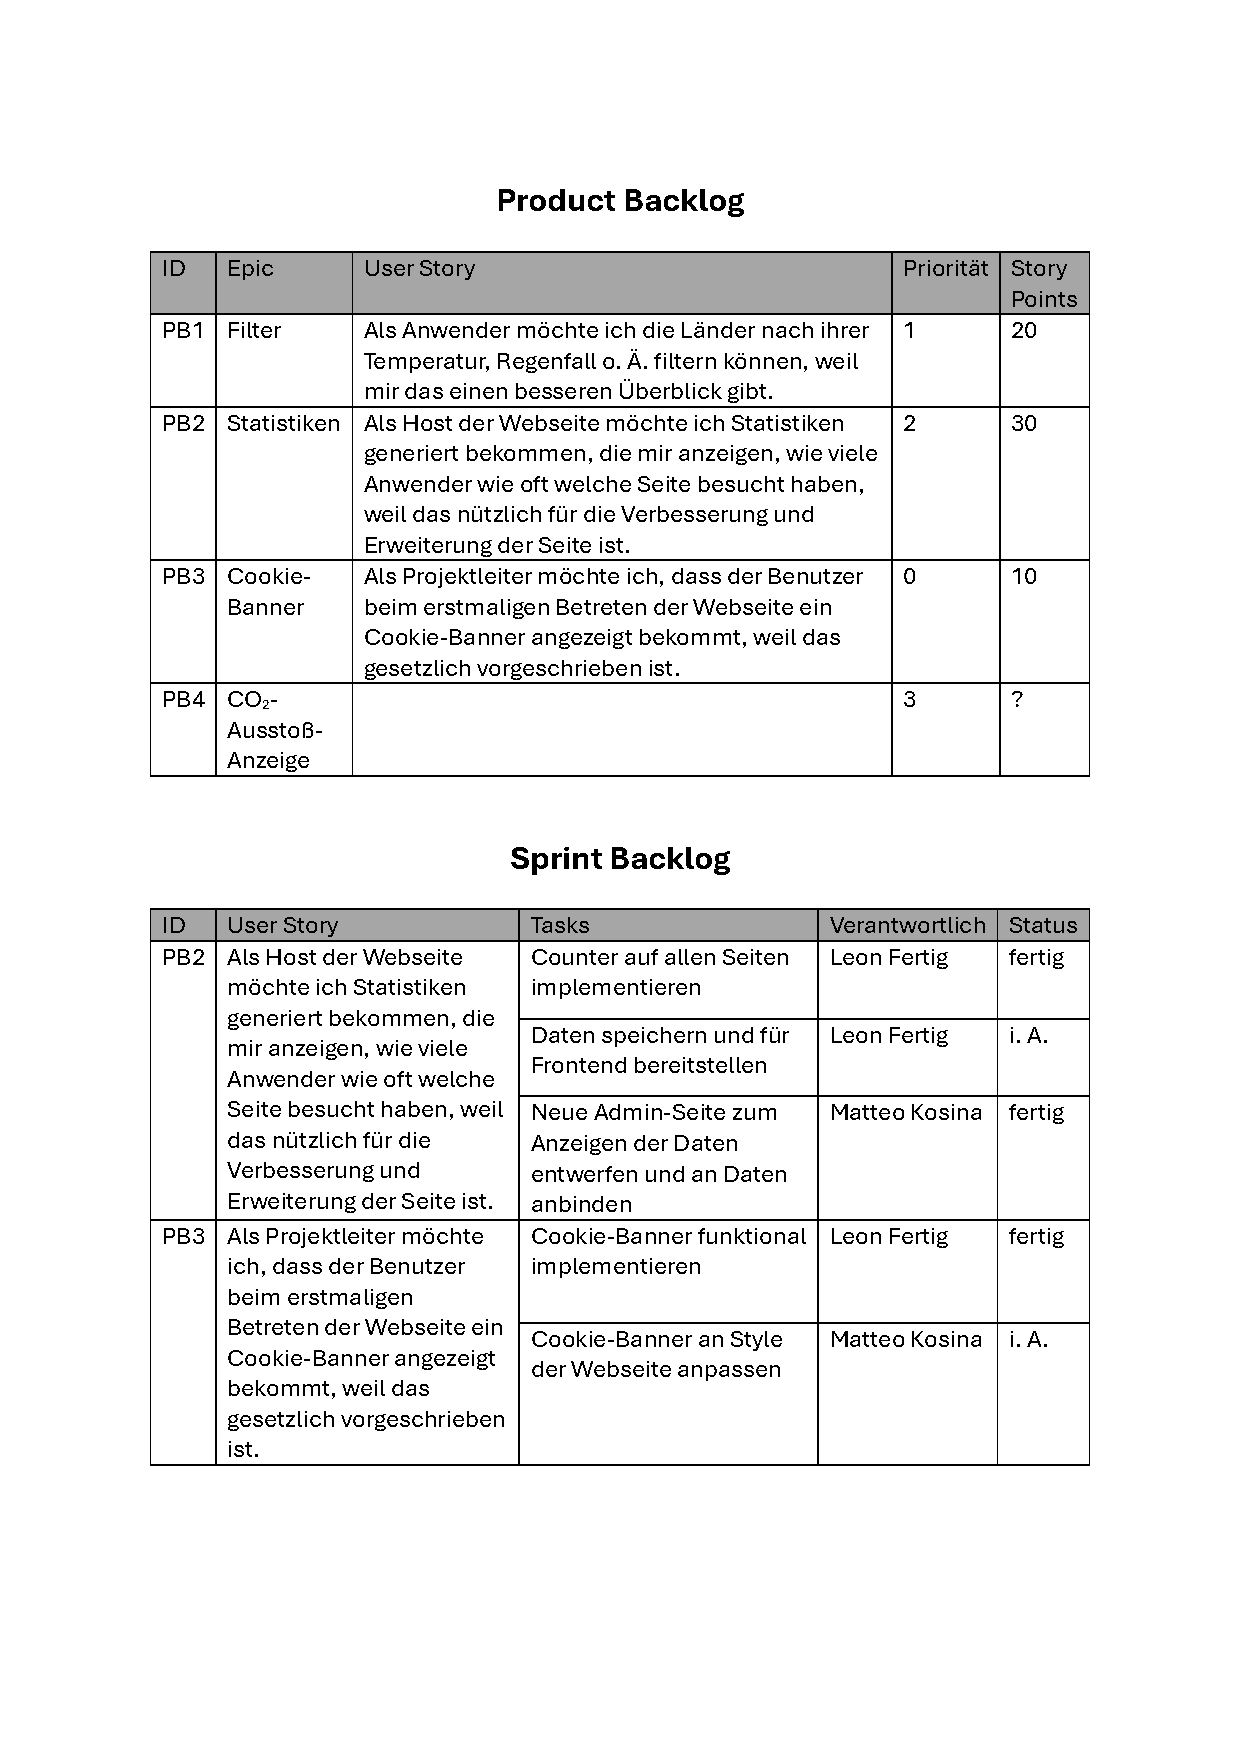
\includegraphics[width=\textwidth]{Planungsdokumente/graphics/Backlog.pdf}

\end{document}
